\documentclass[12pt,prb,aps,epsf]{article}
\usepackage[utf8]{inputenc}
\usepackage{amsmath}
\usepackage{amsfonts}
\usepackage{amssymb}
\usepackage{graphicx} 
\usepackage{latexsym} 
\usepackage[toc,page]{appendix}
\usepackage{listings}
\usepackage{xcolor}
\usepackage{soul}
\usepackage[T1]{fontenc}
\usepackage{amsthm}
\usepackage{mathtools}
\usepackage{setspace}
\usepackage{array,multirow,makecell}
\usepackage{geometry}
\usepackage{textcomp}
\usepackage{float}
%\usepackage{siunitx}
\usepackage{cancel}
%\usepackage{tikz}
%\usetikzlibrary{calc, shapes, backgrounds, arrows, decorations.pathmorphing, positioning, fit, petri, tikzmark}
\usepackage{here}
\usepackage{titlesec}
%\usepackage{bm}
\usepackage{bbold}

\geometry{hmargin=2cm,vmargin=2cm}

\begin{document}
	
	\title{LC 10 Du macroscopique aux microscopique dans les synthèses organiques}
	\author{Naïmo Davier}
	\date{Agrégation 2019}
	
	\maketitle
	
	\tableofcontents
	
	\pagebreak
	
\subsection{Introduction}
	\textbf{Pré-requis} : chaines carbonée, méthodes de représentation des molécules, groupement caractéristique en chimie organique, liaisons polarisées.\\
	
	On a la nécessité de connaître les réactifs et les mécaniques qui composent les réactions afin de les utiliser et optimiser, notamment dans l'industrie.
	
\section{Aspect macroscopique}
%\subsection{Identification}
%Tableau décrivant les différents groupes caractéristiques en chimie orga. Chaque groupe conduit à des comportements particulier, leur identification est donc essentielle pour comprendre comment les molécules vont réagir.\\

%Exemple de la molécule d'aspirine : formule topologique, identification des groupes caractéristiques : ester + ac carboxylique.\\

%Structure de la nomenclature : [préfixe][radical][suffixe].\\
%Exemple (acide 3-éthyl-2-oxobutanoïque), dans lequel on explicite la règle de numérotation des carbones dans les chaines carbonées. On voit que cela permet d'identifier précisément toutes les molécules, notamment de chimie organiques.
\subsection{Rappels}
En chimie organiques on traite des molécules ayant des squelettes carbonés, habillés essentiellement d'hydrogène : ces deux éléments sont centraux en chimie organique. Les autres éléments sont appelés hétéroatomes et seulement un petit groupe joue un rôle important : l'oxygène, l'azote, les halogènes, le soufre, le phosphore et quelques éléments métalliques. Les liaisons formées entre un atome de carbone et un hétéroatome ou un groupe sont souvent polarisées, et peuvent ainsi se rompre de manière asymétrique, et plus ou moins spontanément. On va voir que cela mène à différents mécanismes qui gouvernent les différentes réactions en chimie organique.

\subsection{Catégories de réaction}
\textbf{B.Fosset} \textit{Chimie tout en un PCSI} chapitres 9 et 10.

\subsubsection{Substitution}
\textbf{Exemple : }
\begin{eqnarray}
&CH_3&\hspace{3.8cm} CH_3\\
&|& \hspace{4.1cm} | \\
CH_3&-C-&Cl + H_2O \; = \; CH_3-C-OH + H^++Cl^- \\
&|&\hspace{4.1cm} |\\
&CH_3&\hspace{3.8cm} CH_3
\end{eqnarray}
on parle de substitution lorsqu'il y a remplacement d'un atome ou un groupe d'atome, ici le groupe hydroxyde est remplacé par l'atome de Chlore. %C'est un groupe nucléophile qui se substitue à un groupe nucléofuge. Cette réaction est possible ici parce que la liaison $C-Cl$ est polarisée : le doublet est plus attiré par l'atome de chlore, qui va donc partir avec et laisser la place au groupe hydroxyde qui va venir combler le manque d'électron qui est apparu sur le carbone.

\subsubsection{Addition}
On parle d'addition lorsque un carbone insaturé voit sa double liaison se rompre pour accueillir un nouveau groupe (nucléophile), comme par exemple
\begin{eqnarray}
CH_3-CH=O + H_2 \longrightarrow CH_3-CH_2-OH
\end{eqnarray}

\subsubsection{Élimination}
On parle d'élimination lorsque deux groupes portés par des carbones voisins sont retirés d’une molécule sans arrivée d’autres
groupes d’atomes. Il se forme alors une liaison multiple. Voici un exemple

\begin{figure}[h]
\centering 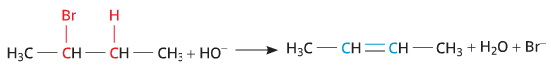
\includegraphics[width=15cm]{elimination.png}
\end{figure}


Les réactions élémentaires que l'on vient de voir semblent ad-hoc, on ne comprend pas à première vue comment elles s'articulent exactement... On va maintenant regarder ce qui se passe à l'échelle microscopique et introduire notamment deux notions qui vont nous permettre d'y voir plus clair.


\section{Aspect microscopique}

\subsection{Polarisation}

Notion d'électronégativité, il existe des atomes plus électronégatifs que d'autres. On peut en déduire que les liaisons peuvent êtres polarisées, introduire la notation $\delta^{\pm}$ avec les exemples $H_2$, $C-C$ pour les liaisons non polarisées et $HCl$, $OH$ pour les liaisons polarisées.

\subsection{Site donner ou récepteur}

On parlera de groupe nucléophile pour un groupe qui "aime les noyaux" : c'est à dire qui peut fournir des électrons tel que $OH^-$ par exemple, et de groupe électrophile pour une groupe qui attire les électrons, qui peut accepter des électrons comme un carbone insaturé, un cation ou $H_3O^+$ par exemple.
	
\subsection{Mécanisme de réaction}
On schématise les réactions élémentaires à l'aide de flèche indiquant la dynamique des doublets électroniques. Illustrer avec les 3 réactions choisies pour les présenter les mécanismes réactionnels.


\section{Synthèse de l'aspirine}
\textbf{Le maréchal} \textit{ Tome 2 p151}\\
Schéma de la réaction, ne faire que la cristallisation et la caractérisation du produit en direct. Évaluer si le produit obtenu est pur ou si il reste de acide salicylique : test visuel et point de fusion. Calcul du rendement.\\
\textbf{Attention : la solution à cristalliser obtenue en préparation peut prendre en masse au contact de l'air en refroidissant, il ne sera plus possible de la passer au Buchner dans ce cas}\\

\textbf{Mécanisme réactionnel de la synthèse de l'aspirine} très bien présenté dans le poly de \textbf{Pierre Henry Suet} :
\begin{figure}[h]
	\centering 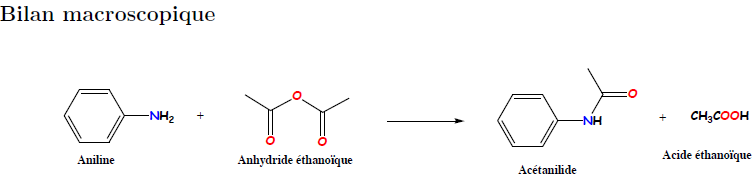
\includegraphics[width=16cm]{aspi_macro}
\end{figure}
\subsubsection{Mécanisme réactionnel}

\begin{figure}[h!]
	\centering 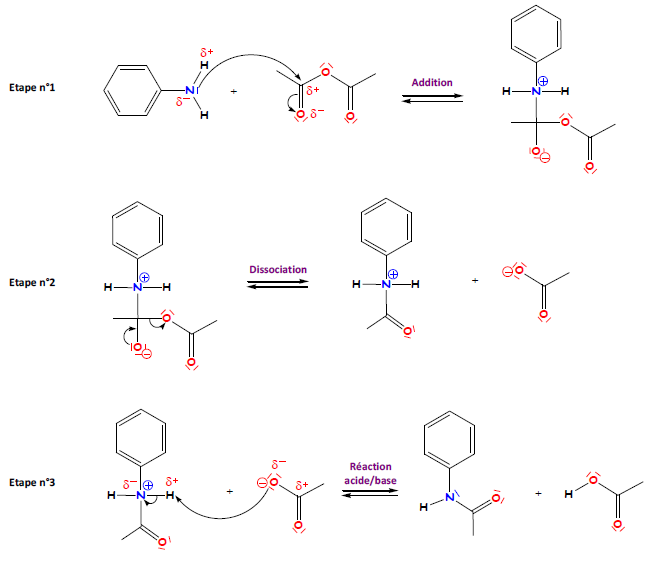
\includegraphics[width=14cm]{aspi_mecanisme_reac}
\end{figure}
\section{Conclusion}
On a montré qu'il était possible d'étudier les mécanismes à l'échelle macroscopique comme microscopique. Cela permet notamment de comprendre la cinétique de ces réactions.

\section*{Questions}
Avant de classer les réactions dans les catégories représentées, quelles sont les deux grandes familles de réactions ?\\
Modification de la/des fonction(s) ou modification de la chaîne carbonée.\\

A la quelle de ces deux familles appartient la synthèse de l'aspirine ?\\
C'est une modification de fonctions.\\

Pourriez vous définir clairement et simplement une réaction d'addition ?\\
On diminue le nombre d'insaturations.\\

De quel type de réaction il s'agit dans le cas de $C_4H_9-OH + H-Cl =...$ ?\\
On regarde quels sont les atomes les plus électronégatifs, ce sont $O$ et $Cl$, $O$ va attirer le proton de l'acide chlorhydrique, on a alors $H_2O$ qui est un bon groupe partant et va ainsi former un carbanion qui sera attaqué par $Cl^-$. C'est donc un mécanisme \textbf{SN$_1$}.\\

Quel sont les mécanismes en jeu dans la synthèse de l'aspirine ?\\
Addition suivie d'une élimination.\\

Comment savoir si un atome est électronégatif ? Quels sont les cas les plus fréquents ?\\
En haut à droite dans le tableau périodique. $O$, $N$, $Cl$...\\

Quels sont les réactifs de Grignard ?\\
ex : organomagnésiens.\\

Comment s'appelle un composé accepteur d'électrons ?\\
Un électrophile.

\section{Remarques}
L'identification ne fait pas partie de cette leçon, le mettre en prérequis, et bien nommer le groupes tout de même à chaque exemple.\\
Il faut traiter les modifications de chaîne et modification de fonctions.\\
Il faut expliquer na notion de flèche, c'est la première fois que l'on voit cette notion. Il faut bien faire chaque étape sans en sauter.\\
On peut passer plus de temps sur les liaisons polarisées, parler d'hétéro atomes.\\
Regarder le programme de terminale STL option SPCL.\\
On ne fait plus de test chimique en général : enlever le test de la fonction phénol pour caractériser l'aspirine.\\
Le mécanisme est plus simple à décrire si l'on fait la synthèse d'un savon, ou la saponification d'un ester.\\


\begin{figure}[h]
	\centering 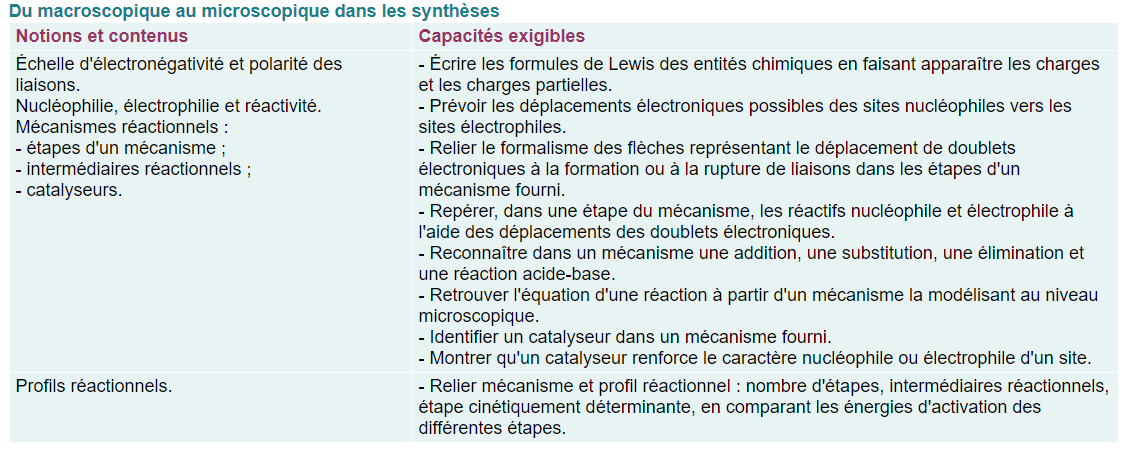
\includegraphics[width=18cm]{programme_Tle_SPCL}
	\caption{Programme terminale STL option SPCL}
\end{figure}

\end{document}